\svnkwsave{$RepoFile: siminos/chapter/spatiotemp/blogAC.tex $}
\svnidlong {$HeadURL: svn://zero.physics.gatech.edu/siminos/spatiotemp/chapter/blogAC.tex $}
{$LastChangedDate: 2019-05-15 14:46:03 -0400 (Wed, 15 May 2019) $}
{$LastChangedRevision: 6812 $} {$LastChangedBy: predrag $}
\svnid{$Id: blogAC.tex 6812 2019-03-20 21:42:41Z predrag $}

\chapter{Andy Chen: Fall 2017 notes}
\label{chap:blogAC}
% Predrag                                           26 May 2016

\bigskip

\hfill {\large Andy Chen <achen87@gatech.edu >}

   % *********************************************************************
\hfill   {\color{red} The latest entry at the bottom for this file / chapter}

\section{Fall 2017 project description}

\begin{description}

    \PCpost{2017-08-23}{
The expected part - to complete the project successfully - is to

\begin{description}
%  \item[[ ]] 2016-05-22 went through plane Couette
%  \HREF{http://ChaosBook.org/tutorials} {tutorial}
  \item[[ ]]
Understand our formulation of search for spatiotemporally periodic solutions
of the 1D Kuramoto Sivashinsky equation, learn how to use Matt's codes, and
numerically reproduce his \KS\ solutions for
several finite $L\times T]$ spatiotemporally doubly-periodic domains (\twots).
  \item[[ ]]
Report on your progress at least once weekly by entering detailed blog posts
of your progress, both in learning the subject (what have you learned by
studying such and such publication) and in recording your progress (successful
and unsuccessful numerical calculations, what insights were needed to fix
them. Matt will teach you how, he is very good in blogging his progress.
  \item[[ ]]
Determine
by the end of the semester at least one (but hopefully many:) new
solution that we do not have already in our database.
  \item[[ ]]
Deliver by the end of semester the project report (for examples, see
ChaosBook.org/projects).
\end{description}

\bigskip

Optional things you might want to do, to gain a deeper understanding:
\begin{description}
  \item[[ ]] Read ChaosBook.org chapter
\HREF{http://ChaosBook.org/paper.shtml\#PDEs}{Turbulence?},
critically (with comment for Predrag to improve it)!
It aims to explain the relation between $L$ and the hyperviscosity
$\nu$, and it should be the fastest introduction to \KSe, for our
purposes, so blog %in \refsect{c-PDEs}
about what is unclear and what is missing.
% mark this box once you have entered a summary in \refsect{c-PDEs}
  \item[[ ]] \KS\ description in \refsect{sect:KStimeInt}
  \HREF{http://chaosbook.org/course1/Course2w16.html} {Course 2, week 16}
  might also be helpful.
  \item[[ ]] derive Michelson\rf{Mks86} ODEs and reproduce numerically
  some \eqva\ and \reqva\ for the $T=0$, spatially infinite domain
  \item[[ ]] Reading part of the project:
The best papers on $T=0$ seem to be
\begin{description}
  \item[[ ]] Michelson\rf{Mks86}
  \item[[ ]] Lan and Cvitanovi{\'c}\rf{lanCvit07}, summarize it here in
\refsect{sect:KSeqva}
  \item[[ ]] Lan\rf{LanThesis} thesis, summarize it here in
\refsect{sect:KSeqva}
  \item[[ ]] understand Dong and Lan\rf{DoLa14} {\em Organization of
  spatially periodic solutions of the steady {Kuramoto–Sivashinsky}
  equation} in detail, summarize it here in \refsect{sect:DoLa14}.
\end{description}
check off the boxes once you have read the above sources
and entered material learned from them either here, or in separate
sections (one for each source, as, for example, \refsect{sect:DoLa14})
  \item[[ ]] summarize $T=0$ in \refsect{sect:KSeqva}
  \item[[ ]] write a code that solves
 \KS\ evolution forward in space for finite $T$ periodic, spatially infinite domain
 (see \refsect{sect:KSspaceInt}; ask Burak for help)
  \item[[ ]] discuss the patterns that you see
  \item[[ ]] describe at length the $T\neq0$ results in \refsect{sect:KSspaceInt}
\end{description}
Andy, check off the boxes, with the date, as you complete them.
That, written up in your blog (this \emph{blogAC.tex} file), is good
enough for the completion of the Fall 2017 term project.
    }

    \PCpost{2017-08-23}{
For this project you are not expected to do original research - it's meant to
be an undergraduate training, but if you have time, there could also be
a bonus part:
If, in addition, you
\begin{description}
  \item[[ ]]
If you write new code, contribute to developing the theory, it would be
wonderful, and sometime this can lead to a publication (see
ChaosBook.org/projects/pubs.html)
  \item[[ ]] write up a literature survey
  \item[[ ]] compute any (by definition, new) {\po}s and/or {\rpo}s
for a fixed finite $T$ time-periodic spatial strip
  \item[[ ]] reduce the \On{2} symmetry of the \eqv\ equations
  \item[[ ]] there should be
also solutions that belong to invariant subspaces, much group-theoretical
analysis not done yet (that would mean that there are all kinds of
important \reqva\ that the literature has missed)
\end{description}
Such contributions are likely worth a publication.

But you have a heavy course load, and your courses take priority.
And, always! get enough sleep.
    }

\end{description}

\section{Andy's blog}
\label{sect:blogAndy}

   % *********************************************************************
\hfill   {\color{red} The latest entry at the bottom of this blog}

\begin{description}

%     \ACpost{2017-08-23}{
% Here is an example of \ACedit{text edit by me},
% and here one of a footnote by me\AC{2017-08-23}{test footnote}.
%    }

%     \ACpost{2017-08-23}{My \\
% SVN repo is {\em svn://zero.physics.gatech.edu/siminos}
% \\
% userID is
% \texttt{achen87}, the password is \texttt{spatioTemp}

% folders are in \texttt{siminos/chen/}
% \begin{itemize}
%   \item[python/]
%   \item[matlab/]
%   \item[presentations/]
%   \item[projectFall17/]
% \end{itemize}
% Predrag recommends that I keep \texttt{00ReadMe.txt}'s up to date,
% with descriptions of what program does what, etc...
%     }

    \ACpost{2017-08-23}{
Discussion with Predrag and Matt, \KS\ \eqva\ and \reqva\ project Fall 2017:
\begin{itemize}
\item blog the project progress here
\item blog whatever I'm reading and learning about
    dynamical systems here
\end{itemize}
    }

\PCpost{2017-08-23}{to Andy:
%Everything from here on is copied from Matt's blog, and you want to delete
%it. I kept it here just so you can se how some pieces of LaTeX code work. In
%any case,
Scan through Matt's blog \refchap{chap:blogAC}, especially the beginning,
for useful pointers how to start and what to study...
   }


\PCpost{2017-08-24}{
% It would be easier (and faster in the long run) to do this on the
% CNS linux cluster. Your userID is \emph{achen87}, I emailed you the password separately.

You can use the linux box in the second bay to the left in
the grad students office W503,
or linux terminal in the computer cubicle W508E (Matt has the key),
Login as \emph{achen87}. Then  -if you are not logged into hard.physics-
\\
\emph{ssh -X achen87@hard.physics.gatech.edu}
\\
that puts you into
(former) Xiong's
linux box which has all the packages you need already installed.
If you start generating lots of data, store it locally, somewhere in
\emph{hard.physics.gatech.edu:/usr/local/home/achen87/}

You can get there by \emph{cd localHard}. That is needed because your
home directory is backed up every night, and if there are
President Rump-self-perception size files in it, it will break the backup for
everyone.

 If not using a CNS linux box,
 \HREF{http://www.cns.gatech.edu/CNS-only/VPN.html}{VPN} to get past the
 firewall. Then \\
 \emph{ssh -X achen87@zero.physics.gatech.edu}
 \\From there,\\
 \emph{ssh -X achen87@hard.physics.gatech.edu}
 \\
 This \emph{-X} enables you to open
 the \emph{hard.physics.gatech.edu} Matlab etc. on your own laptop, provided ...
 (simpler you talk to Matt about it).
     }


\MNGpost{2017-08-25}{:
Andy here are some references for the numerical methods used for time integration,
SO(2) symmetry reduction, and a couple papers on finding spatiotemporal solutions.
\begin{itemize}
  \item Spatiotemporal papers\rf{WGBGQ13,lop05rel}
  \item Numerical methods: Time-integrator\rf{ks05com}
  \item Direct-matrix methods\rf{Chu09}
  \item \SOn{2}\ symmetry reduction: Budanur \etal\rf{BudCvi14}
  \item Spatiotemporal blog in the SVN  repository \texttt{dasbuch}
\end{itemize}
I would focus on \wwwcb\ and then the blog as that is
the best general resource around, especially the chapter
\HREF{http://ChaosBook.org/paper.shtml\#PDEs}{Turbulence?}.

The next in terms of priority is Kassam and Trefethen\rf{ks05com} for the
numerical integration, and the Budanur, Cvitanovi\'c, Davidchack, and Siminos
2015 article\rf{BudCvi14} for how we quotient the spatial translation
symmetry of the \KSe.
}

\ACpost{2017-08-25}
{
  SVN checked out all folders and files in the directory
  \\
  zero.physics.gatech.edu:/home/chen/siminos/ onto my laptop
}

\ACpost{2017-08-28}
{
Read through MNGkstorifunc\_rfft.py and MNGkstori.py:
\begin{itemize}
  \item Refamiliarized myself with Newton's Method and Fourier Transforms
  \item Read about FFT, RFFT, iRFFT, HDF5 files, and the Kronecker product
\end{itemize}
}

\ACpost{2017-08-30}
{
Began reading Chapter
  \HREF{http://ChaosBook.org/paper.shtml\#PDEs} {Turbulence?} from ChaosBook
}

\ACpost{2017-09-06}
{ :
\begin{description}
\item[Meeting with Matt]
Discussed the code that attempts to locate initial
conditions for the spatiotemporal code. Matt has been translating the MATLAB
code into python and is almost done with the initial condition locator.

The exponential time differencing Runge-Kutta 4th order (ETDRK4) code takes a
point in hyperspace and evolves it through time to find {\ppo}s.
This point can either be retrieved from a file or generated by the python
script itself. Each iteration generates a Poincar\'e plane containing the
initial point and evolves the system while searching for close orbits: if the
point evolves back to the general location of the initial point and crosses
the Poincar\'e plane, the initial point is recorded as a promising input
candidate for the spatiotemporal code.

To perform the time evolution, ETDRK4 increments time and finds solutions to
the KS equation. When a possible orbit is found, the script performs FFT to
``clean up'' the orbit: high frequency coefficients are discarded so that the
orbit becomes periodic. However, discarding terms should be done carefully:
eliminating too many terms may drastically change the location of the orbit in
{\statesp}.

\item[{\Ppo} vs {\rpo}]
{\Ppo} orbit refers to solutions found by the ETDRK4
code. These orbits exhibit periodic ``mirroring'' in a t-x plot (not sure what
this mirroring is). Relative periodic orbit refers to orbits that lie on a t-x
torus (still not sure exactly how this works) such that the path traced by the
orbit corresponds to a t-x plot that repeats itself but each cycle may be
offset in position.

\item[Ch 30: Turbulence?]
Page 573 talks about {\rpo} vs {\ppo}. It seems that
{\ppo}s are more symmetric than {\rpo}s: any shift accumulated in the first orbit
will be compensated by shifts in later orbits, thus bringing the solution back
to the initial condition.
\end{description}
}

\ACpost{2017-09-08}
{ :
\begin{description}
  \item[Space groups]
Space groups most often refer to symmetry groups in 3D space (though many
texts refer to 2D case as space groups as well). The operations include
reflection, rotation, improper rotation (roto-reflection), screw axis, and
glide plane.
  \item[Wallpaper groups]
These are the space group analogs in 2D. There are 17 distinct groups, but
colors can be added / removed to decrease / increase the number of symmetry
operations. In to 2 dimensions translation, rotation, reflection, and glide
reflection are valid operations in the group. Frieze groups are subset of 2D
patterns that exhibit 1D properties: they can be visualized as a line with
tick marks on each side.
  \item[Symmetry groups in 1D]
Reflection and translation are the only symmetry operations in 1D. A special
type of reflection (``negative reflection'') is produced when the reflection
of a 2-colored 1D object results in the negative image of the original.
Perhaps time reversal can be interpreted as such 1D symmetry group.
\end{description}
}

    \PCpost{2017-09-08}{
In the long run (for later, when you revisit your notes to write up the
project report) to refer now to the literature that you found useful, and are
reading right now. Let's say Dresselhaus \etal\rf{Dresselhaus07}, if that's
where you got the above information from.
    }

    \PCpost{2017-09-12}{
My draft of the paper that Matt and I should write starts with the above
\refchap{chap:spatiotemp} {\em Space-time, sliced \& sectioned}. I recommend
you read it, it should motivate the whole project. And feel totally free to
clip \& paste whatever from this text into the introduction of your project,
\refchap{chap:reportAC}~{\em Spatiotemporal solutions of \KSe} (a tentative
title).
    }

\ACpost{2017-09-18}
{ Studying
{\bf Plane Couette Tutorial}
The information available in plane Couette
\HREF{http://ChaosBook.org/tutorials}{tutorial} explained the {\statesp}
simulations for the Navier-Stokes equation. It is mentioned that the
simulations are run in full (61506 dimensional) {\statesp}, but this work
is not considered modeling(?). The NS equations for plane Couette flow are
equivariant under ``shift-reflect'' and ``shift-rotate'' transformations where
exact invariant solutions include equilibria and periodic orbits. Even if the
initial state of the fluid is not in an invariant subspace, the turbulent
dynamics stay close to invariant subspace terbulence at all times. This is
most likely analagous to the attractors in KS that Matt mentioned.

Exact solutions of NS include the classic laminar equilibrium, Nagata lower
and upper equilibria (two branches resulting from bifurcation in bulk
dissipation rate ($D$) vs Re plot), and others. When Re is large, high $D$
curves become more unstable so we usually look at the low $D$ ones. Solutions
also have preferred wavelengths determined by the wall separation distance and
can form a orthonormal basis. However, there are usually only 4 ``vectors''
(is the entire 61\,506 dimensional \statesp\ not entirely spanned?).
}
\PCpost{2017-10-02}{\PCedit{
The three or four vectors that we typically construct,
 are vectors in the entire 61\,506 dimensional
\statesp, cleverly chosen so that projection on the small subspace they span
are informative about the structures we are interested in (heteroclinic
connections; visitation of \po s to various regions of the \statesp).
The do not span the entire \statesp.
}}


\ACpost{2017-09-20}
{ :
I have started reading through Michelson\rf{Mks86}. I am still digesting
\refsect{sect:KStimeInt} as well as the info from the plane Couette tutorial
and will start watching the Youtube links in
\HREF{http://chaosbook.org/course1/Course2w16.html}{Course 2, week 16}.

About current \refeq{spatFT} in \refsect{sect:KStimeInt}~{\em \KS\ on a
spatial strip}: indicating that the sums in the first equation are iterating
over $n$ might help clarity.
}

\PCpost{2017-10-02}{ I guess I do not understand ``iterating
over $n$.'' Please rewrite the 0th order draft in your report
\refsect{ACsect:KStimeInt} in such a way that that is clearer?
    }

\ACpost{2017-10-02}{
Should all the derivations be logged in the project
report or blog (or both)?
}

\PCpost{2017-10-02}{
Good - I was getting worried about the silence. My advice for Michelson staff
is to blog / enter into the report draft what formulas you needed to do your
calculations. For example, the KS equation is of different form there (if I
remember correctly, you have to convert it to the form we use), etc. You need
to report sufficient detail so it is clear what you are computing.

It is OK to clip and paste from LaTeX source files - in siminos (all our recent
articles are there) and dasbuch repositories you have most of the stuff
already typed up. Saves time. I can give access to y-lan if you needed.
    }

\ACpost{2017-10-06}
{ :
\begin{description}
\item[{\Ppo} Initial Conditions]
According to Matt, the method of weighting the Fourier coefficients on a
Gaussian distribution centered around the first few terms does not work as well
as we hoped. He is continuing on the adjoint method while I continue to work
through the literature.

\item[Michelson1986]
Using the difference method, the \KSe\ \refeq{eq:ksmich1} can be approximated by
\begin{equation}
    \frac{(y_{j+3} - 3 y_{j+2} + y_{j+1} - y_j)}{\Delta x^3} + \frac{y_{j+2} - y_{j+1}}{\Delta x} = c^2 - \frac{y_{j+2}^2 + y_{j+1}^2}{4}.
\end{equation}
The derivation can be found in my project report (how should I cite it?). I'm
not sure why the nonlinear squared term neglects the mixed term $\frac{1}{2} y_0 y_1$ if
its intended approximation is of the form $[\frac{1}{2} (y_0 + y_1)]^2$. The paper might
discuss the solution to this problem and I just haven't found it yet (I will keep
searching and thinking about it). The paper also uses the initial condition $y(0) = 0$,
but the difference method requires at least three points before it can go through
the iterative process of convergence. Michelson establishes a new parameter $s$ such
that the neighboring $y$ points of $y_0$ are scaled directly to the step size of $x$:
$y_1 = -y_{-1} = \Delta x \cdot s$. To find a suitable $s$, an upper bound $y_{\text{max}}$
is defined such that we can keep track of $x_{\text{max}}(s) = x_j = j \Delta x$ where $j$
is the index of $y_j$ at the first occurrence of $|y_j| \geq y_{\text{max}}$.

I am currently trying to replicate the solutions that Michelson found with $y_max = 10$ and
$\Delta x = 0.05$. His paper bounds $c$ to the interval $[0,4]$ so I might try to run a sweep
after producing some of the result he found with his $c$ values.

Since the solution equation has the speed parameter of $c^2$, does this mean
that two solutions exist for each set of steady system differing only in the
direction of propagation?

In comparison to the \KSe\ used in \HREF{http://ChaosBook.org/paper.shtml\#PDEs}{Turbulence?},
Michelson remains true to the original equation without the viscosity term on the fourth
spatial derivative of $u$. I'm still not quite sure how to include the viscosity term, but I'm
looking into it.

\end{description}
}

\ACpost{2017-10-11}
{ :
\begin{description}
\item[Michelson1986]
I'm still working through the Numerical Experiments section and trying to
understand the proof for $s$ bounds of solutions. The python script runs
smoothly, spitting out the $y_{\text{max}}$ for any given $s$ and $c$ parameter,
so I just need to understand which $s$ to use. The paper mentions that solutions
can be found with a parameter $s$ that corresponds to a local maxima in the
function $x_{\text{max}}(s)$. I see maxima when using a step size of 1 for $s$.
I will be testing for smaller step sizes and see if the peaks are actual
maxima or discontinuities.

\end{description}
}

\ACpost{2017-10-13}
{ :
\begin{description}
\item[Michelson1986]
Starting from Equation 30.1 in \HREF{http://ChaosBook.org/paper.shtml\#PDEs}{Turbulence?}
which includes density $\rho$ and viscosity $\nu$ terms. To arrive at Equation 30.4, the
viscosity is scaled out by rescaling the interval of $x$:
\begin{equation}
    x \in [0,L] \to [0,L \nu^{-1/2}].
\end{equation}
Predrag mentioned including the viscosity term in the code for generating Michelson's
solutions, but wouldn't the scaling caused by viscosity just be reflected in the scaling
of the $x$-axis when plotting $xy$? If so, then the general shape of curves in any
$yy'$ plots would be unaffected by the viscosity value.

I'm still trying to understand the data that the python code is giving me and how to find
the bounded solutions. During the testing of the current code, I have found a discontinuity
in $x_{\text{max}}$ at $c=1.8$ and $s \in [-11.4865655,-11.48656525]$. It's probably
nothing of interest, but I'm still excited something is working. The code currently only
iterates in the positive $y$ direction. I guess I could go backwards into the negative $y$
direction, but I'm not sure if it'll be any more helpful at this stage (maybe in the
future).

I'm still trying to figure out where to go after finding these $x_{\text{max}}$ extrema,
but after reviewing the spectral methods that Matt showed me and from Chapter 4 of the blog
I'm not sure how the nonlinear term works (I'll ask him about it next time). It has also
been a while since I worked with fourth order Runge-Kutta so refreshing myself was a
nice trip down memory lane.

\end{description}
}

\ACpost{2017-10-16}
{ :
\begin{description}
\item[Meeting with Matt]
I talked to Matt about the nonlinear term in the spectral method and it works exactly
as described in \HREF{http://ChaosBook.org/paper.shtml\#PDEs}{Turbulence?}: the coefficients
are taken to configuration space where they are squared, and then the terms are returned
back to Fourier space.

\item[Michelson1986]
Plots of the $xy$ curves look remarkably similar to those in Michelson's
paper (will refine and attach next time)! For $s \in [-5,5]$ and $c \in
[1.210,1.300]$, some curves exhibit many cycles of periodicity, thus
representing trajectories near spatially periodic \eqva. I'll also look into
using the spectral methods for the solution rather than using finite
difference.
%     \PC{2017-12-11}{
% Andy had referred in the previous draft to ``stable periodic orbits.'' Aren't
% all these spatial \eqva\ violently unstable? Ask Matt.
%     }

\end{description}
}

\ACpost{2017-10-18}
{ :
\begin{description}
\item[Michelson1986]
Michelson's paper talks about a solution at $c=1.266$. During my sweep for $c$ and $s$ values
that indicate the general location of periodic orbits, I eventually narrowed my search down to
$c=1.266$ and $s \in [1.330,1.400]$. At $s=1.369$, an orbit with several periods is found
(c.f.\ Fig. 5.1 and 5.2). This $s$ value is isolated from another nearby range of $[1.372,1.389]$
where the orbit has a significant number of periods before diverging.

\begin{figure}[h!]
  \centering
  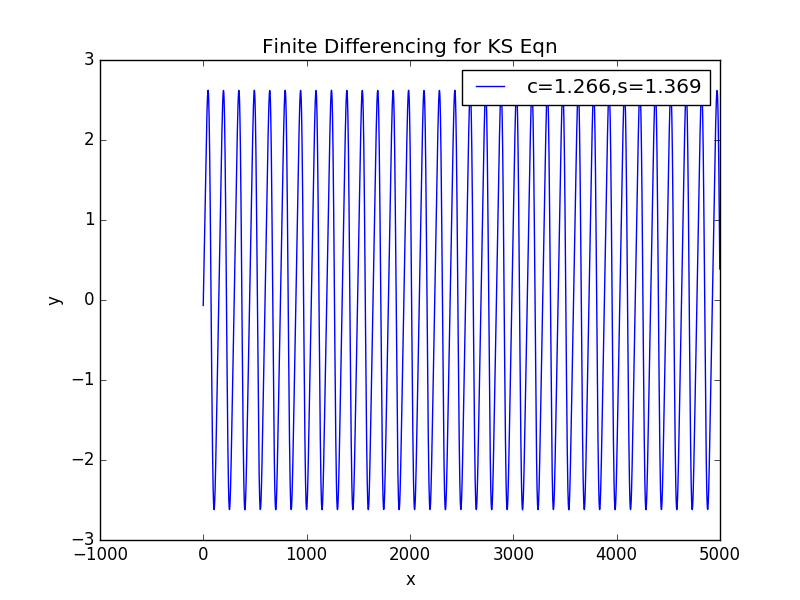
\includegraphics[scale=0.5]{ACxyplotc1266s1369.png}
  \caption{
$(xy)$ plot. The trajectory generated through a finite difference scheme
outlined in Michelson\rf{Mks86} for $c=1.266$ and $s=1.369$.}

  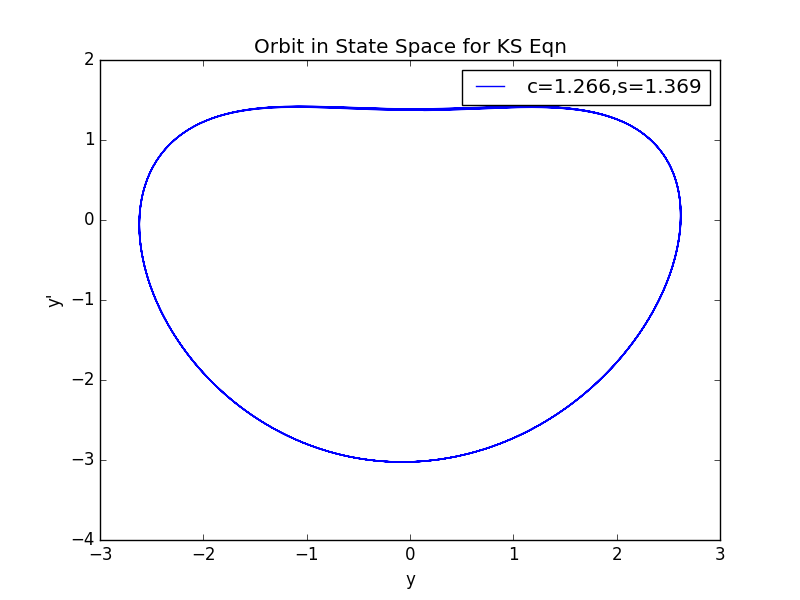
\includegraphics[scale=0.5]{ACorbitc1266s1369.png}
  \caption{\Statesp\ plot. The near-periodic orbit generated through a finite difference
  scheme outlined in Michelson\rf{Mks86} for $c=1.266$ and $s=1.369$.}
\end{figure}

Matt talked to me about a shooting method detailed in Chapter 16.2 of the ChaosBook to refine the
quasi-periodic (?) orbit into an true periodic orbit. I'll read up on that and figure out how to
implement it. Alternatively, Predrag suggested using variational methods to clean up the orbit: a
paper by Dong-Lan goes through the process for finite difference method. Once I get that done, I
might sweep through a different range of $c$ to find more signs of orbits.

We also concluded that the $s$ parameter in the finite difference method
sets the initial conditions for the first and second derivative for the start of the iteration
process. Since the initial condition $y_{-1} = y_{1} = \Delta x \cdot s$ sets the solution as an
even function, I should get the same orbit traveling in the opposite direction if I iterate through
the finite difference scheme in the negative $x$ direction. This entire process will be outlined in
the project report.

\end{description}
}

\ACpost{2017-11-15}
{ :
\begin{description}
\item[Yang15]
The author attempts to obtain time-periodic solutions rather than spatially periodic
ones. Yang's method uses the PDE framework to compute solutions, allowing the system's
structure to be retained and its adjoint to be calculated analytically. It also incorporates
conjugate-gradient method for its computational speed.

The parameters used in the equations are computed with the solution itself. Time is
scaled such that a frequency parameter can be expressed in terms of the periodic solution
itself through a Rayleigh-like quotient:
\begin{equation}
    \omega = \frac{\left< \mathbf{u}_{\tau}, \mathbf{F} \right>}{\left< \mathbf{u}_{\tau}, \mathbf{u}_{\tau} \right>}.
\end{equation}
Matt mentioned that we should consider scaling the space domain instead, but having both
space and time as variables will require some tinkering with Yang's code.

Furthermore, the author arrives at an integrodifferential equation and solves it by the
Newton-CG method:
\begin{equation}
    \mathbf{L}_0 \equiv \frac{\left< \mathbf{u}_{\tau}, \mathbf{F} \right>}{\left< \mathbf{u}_{\tau}, \mathbf{u}_{\tau} \right>} \mathbf{u}_{\tau} - \mathbf{F} = 0.
\end{equation}
Apparently the ''price is worth paying for'', but I will need to continue reading to figure
out what Yang is referring to.

\end{description}
}

\ACpost{2017-11-20}
{ :
\begin{description}
\item[Yang15]
Nevermind the last comment from my last blog post. Yang makes it clear that the \KSe\
can now be expressed only in terms of $u(x,t)$ without the need for $\omega$ anymore.
The PDE is now an equation with both differential terms and integral terms in the form
of inner products. This extra step will probably be unnecessary if we decide to keep
time unscaled.

To solve the integrodifferential equation, Yang uses Newton conjugate-gradient (CG)
method. To solve $Ax = b$ given $A$ and $b$, CG requires $A$ to be a symmetric,
positive semidefinite matrix. The method decomposes the solution $x$ into a combination
of mutually conjugate vectors $p_i$, where $p_i$ and $p_j$ are conjugate if
\begin{equation}
    p_i^{\top} A p_j = 0.
\end{equation}
I think Yang is applying the system of equations solver onto
\begin{equation}
    \mathbf{L}_{1n} \Delta \mathbf{u}_n = -\mathbf{L}_0(\mathbf{u}_n)
\end{equation}
where $\mathbf{L}_{1n}$ is the operator $A$ and $-\mathbf{L}_0(\mathbf{u}_n)$ is the
vector $b$.

For Ginzburg-Landau equations, Yang was able to manipulate the solution into
\begin{equation}
    \omega U_{\tau} + i \mu U = G
\end{equation}
where $G = f(|U|,\mathbf{x} \partial_x) U$. Taking $U$ and $G$ as complex functions,
they can be rewritten as
\begin{equation}
    \left\{
    \begin{array}{l}
	U = u + iv\\
	G = g + ih.
    \end{array}
    \right. \label{eq:blogac1}
\end{equation}
Taking the real and imaginary components of \refeq{eq:blogac1}, we arrive at
\begin{equation}
    \left\{
    \begin{array}{l}
	\omega u_{\tau} - \mu \nu - g = 0\\
	\omega v_{\tau} + \mu u - h = 0,
    \end{array}
    \right.
\end{equation}
and by taking inner products, we can express the parameters as
\begin{equation}
    \left\{
    \begin{array}{l}
	\mu = \frac{\left< v,h \right> - \left< u,g \right>}{2 \left< u,v \right>}\\
	\omega = \frac{\left< u_{\tau},h \right> + \left< v_{\tau},g \right>}{2 \left< u_{\tau},v_{\tau} \right>}.
    \end{array}
    \right.
\end{equation}
Similarly, Matt and I tried to apply Yang's process to the \KSe\ . Since our equation
is real valued, we take the \KSe\ to Fourier space to invoke both real and imaginary
components to the solution. However, we hit a bump in the road when solving for the
parameters since our equation includes a nonlinear term.

We tried to use the energy density from
\HREF{http://ChaosBook.org/paper.shtml\#PDEs}{Turbulence?} of ChaosBook to fix this
problem, but the nonlinear term still presents itself as an obstacle. We are
exploring other methods to continue Yang's procedure.

\end{description}
}

\ACpost{2017-11-29}
{ :
\begin{description}
\item[Yang15]
Matt decided that it would be better to leave the \KSe\ in the space domain
rather than try to manipulate it in Fourier space. By applying the dot product on
the right side of each term in the time reparameterized version
($u_t \to \omega u_{\tau}$) of the \KSe\
\begin{equation}
    \omega u_{\tau} = u u_x - u_{xx} - \nu u_{xxxx}
\end{equation}
with $u$ and $\omega u_{\tau} = -f - \nu u_{xxxx}$, we obtain the parameters
$\omega$ and $\nu$ in terms of the solution itself:
\begin{align}
    \nu &= -\frac{\left< f, u \right>}{\left< u_{xxxx}, u \right>}\\
    \omega^2 &= 1 - \left[ \frac{\left< f, u \right>}{\left< u_{xxxx}, u \right>} \right]^2 = 1 - \nu^2.
\end{align}
The second expression restricts $\nu$ to the domain $[0,1]$, but this interval
includes all the values of $\nu$ that Yang has tested with his other numerical
methods. Now we just need to get the Newton method solver adjusted to find periodic
solutions. I will explore the MATLAB code Yang references in the paper to see
if any of it can be repurposed.

\end{description}
}

\ACpost{2017-12-01}
{ :
\begin{description}
\item[Yang15]
Following Yang's process to arrive at the linearization operator of $\mathbf{L}_0$,
Equation 15, of the paper, I have found
\begin{equation}
    \nu(u + \tilde{u}) = \nu - \frac{\left< \left[f_1 + \nu \partial_x^4 \right] \tilde{u} - \omega u_{\tau}, u \right>}{\left< u_{xxxx}, u \right>} + O(\tilde{u}^2)
\end{equation}
where I used
\begin{equation}
    \mathbf{L}_0 = \omega u_{\tau} + \nu u_{xxxx} + f = 0.
\end{equation}
My result looks similar to Yang's, but the only difference is that I kept the
$\nu$ term out of the function $f$. If we had also included the $\omega$ term
in $f$ such that
\begin{equation}
    f \equiv \omega u_{\tau} + u_{xx} - u u_x,
\end{equation}
then the expression we arrive at for $\nu$ is
\begin{equation}
    \nu(u + \tilde{u}) = \nu - \frac{\left< \left[f_1 + \nu \partial_x^4 \right] \tilde{u}, u \right>}{\left< u_{xxxx}, u \right>} + O(\tilde{u}^2),
\end{equation}
strikingly similar to Yang's Equation 15.

\end{description}
}


\end{description}

%%%%%%%%%%%%%%%%%%%%%%%%%%%%%%%%%%%%%%%%%%%%%%%%%%%%%%%%%%%%%%%%%%%%%%%
\printbibliography[heading=subbibintoc,title={References}]
